\documentclass[tikz]{standalone}

\usepackage[T1]{fontenc}
\usepackage[english]{babel}

\usepackage{tikz, pgfplots}

\usepackage{bm}

\begin{document}
    \pgfplotsset{every axis/.append style={
        font=\footnotesize,
        ytick=\empty,
        xtick=\empty,
        line width=1pt,
        tick style={ultra thin}}
    }
    \pgfplotsset{
        every non boxed x axis/.append style={x axis line style=-},
        every non boxed y axis/.append style={y axis line style=-}
    }
    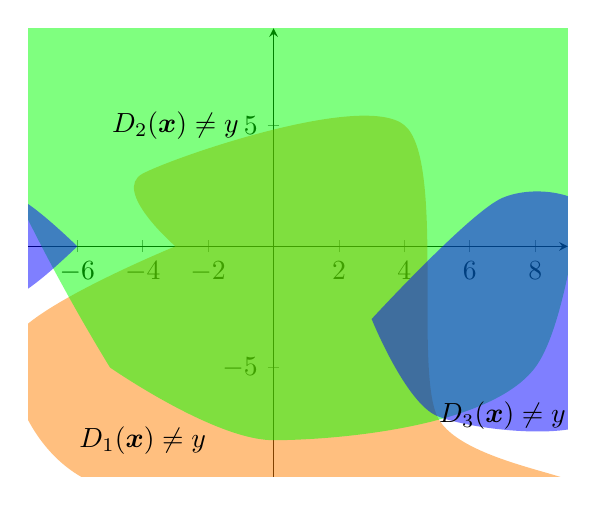
\begin{tikzpicture}
        \begin{axis}[
            axis lines=center,
            ymax=9,
            ymin=-9.5,
            xmax=9,
            xmin=-7.5
        ]
            \addplot [smooth, draw=none, no markers, fill=orange, opacity=.5] coordinates{
            	(-3, 0)
            	(-4, 3)
            	(4, 5)
            	(5, -7)
            	(9, -10)
            	(-5, -10)
            	(-8, -4)
            	(-3, 0)
            } node[black] {};
            \addplot [smooth, draw=none, no markers, fill=green, opacity=.5] coordinates{
            	(-5, -5)
            	(0, -8)
            	(8, -5)
            	(10, 10)
            	(9, 10)
            	(-9, 10)
            	(-5, -5)
            } node[black] {};
            \addplot [smooth, draw=none, no markers, fill=blue, opacity=.5] coordinates{
            	(-6, 0)
            	(-8, -2)
            	(-8, 2)
            	(-6, 0)
            } node[black] {};
            \addplot [smooth, draw=none, no markers, fill=blue, opacity=.5] coordinates{
            	(3, -3)
            	(7, 2)
            	(10, 1)
            	(10, -7)
            	(5, -7)
            	(3, -3)
            } node[black] {};
            \node at (axis cs:-4, -8) {$D_{1}(\bm{x}) \neq y$};
            \node at (axis cs:-3, 5) {$D_{2}(\bm{x}) \neq y$};
            \node at (axis cs:7, -7) {$D_{3}(\bm{x}) \neq y$};
        \end{axis}
    \end{tikzpicture}
\end{document}